%\documentclass[runningheads]{llncs}
\documentclass[conference]{IEEEtran}
%\IEEEoverridecommandlockouts
%
\usepackage{graphicx}
% If possible, figure files should be included in EPS format.
%
\usepackage{amsmath}
%
% If you use the hyperref package, please uncomment the following line
% to display URLs in blue roman font according to Springer's eBook style:
\usepackage{hyperref,xcolor}
\renewcommand\UrlFont{\color{blue}\rmfamily}

\begin{document}
%
\title{Impact of switching bug trackers: a case study on a medium-sized open source project}
%
%\author{Th\'eo Zimmermann\\
%$\Pi R^2$, Inria and
%IRIF, Paris-Diderot University\\
%Paris, France\\
%Email: theo@irif.fr
%\and
%Annal\'i Casanueva Art\'is\thanks{This work was partly funded by El Conacyt of the Mexican government.}\\
%Paris School of Economics\\
%Paris, France}
%
\maketitle
%
\begin{abstract}
For most software projects, the bug tracker is an essential tool. In open source development, this tool plays an even more central role as it is generally open to all users, who are encouraged to test the software and report bugs. Previous studies have highlighted the act of reporting a bug as a first step leading a user to become an active contributor.

The impact of the bug reporting environment on the bug tracking activity is difficult to assess because of the lack of comparison points. In this paper, we take advantage of the switch, from Bugzilla to GitHub, of the bug tracker of Coq, a medium-sized open source project, to evaluate and interpret the impact that such a change can have.

We first report on the switch itself, including the migration of preexisting bug reports. Then we analyze data from before and after the switch using a Regression on Discontinuity analysis, a novel methodology in the context of empirical software engineering. We complete this quantitative analysis with qualitative data from interviews with developers.
We show that the switch induces an increase in bug reporting, particularly from principal developers themselves, and more generally an increased engagement with the bug tracking platform, with more comments by developers and also more external commentators.
\end{abstract}

%The abstract should briefly summarize the contents of the paper in 15--250 words.

\begin{IEEEkeywords}
bug tracker, switch, migration, bug report, issue, GitHub, Bugzilla, open source, data mining, Regression on Discontinuity, interviews
\end{IEEEkeywords}
%
%
%
\section{Introduction}

Bug reporting is an essential part of software development.
In the context of an open source project, the bug reporting and fixing process is generally done on a public bug tracking platform, and, in the absence of paid testers, it depends a lot on the good will of independent users. Therefore, it involves a strong social component.

However, having an open bug tracking system is not enough to get the bugs reported. In addition to the software having enough users, the process of bug reporting must be easy and appealing. Therefore, creating an environment that eases bug reporting and makes it more appealing may lead to an increase in bug reporting activity (from both developers and independent users), which is well associated with an increase in software quality. First, if the software has not changed, receiving more bug reports indicates that more defects have been found, and not a sudden apparition of defects (Linus's Law ``given enough eyeballs, all bugs are shallow''~\cite{raymond1999cathedral,van2009shallow}). Moreover, assuming that developers are equipped to cope with the increased number of incoming reports~\cite{anvik2005coping, davidson2011coping}, even duplicate reports are not necessarily harmful~\cite{Bettenburg2008}. Second, more activity on the bug tracker can also mean users are helping to reproduce bugs, produce traces, etc. and thus are working with the developers to get the bugs fixed~\cite{breu2010information}. More generally, reporting new bugs and discussing existing bug reports has been shown to be an important step on the path to becoming an active contributor of an open source project~\cite{jensen2007role, nakakoji2002evolution, ye2003toward}.

Despite the importance of the bug tracking environment that we have just highlighted, the impact of a change in this environment has rarely been studied. It is generally difficult to compare the number of bug reports in different environments because it is likely to depend  not just on the reporting environment but also on each particular software and its development dynamics, which would make such an analysis not compelling. To do a valid comparison, one would ideally need to compare two bug reporting environments for the same software, used by the same users, to report the same bugs, in the same period. This is of course impossible. A context approaching this ideal scenario would be to compare the number of bug reports of a particular software before and after the switch to a new environment. Yet, substantial changes in the environment of bug reporting (e.g. changes of bug tracker platform) are rare because once a bug tracking platform is in place, any change comes with a significant cost. 

In this paper, we study the case of the Coq proof assistant, a medium-sized open source software project. We use the switch, from Bugzilla to GitHub, of the project's bug tracker, to analyze how a change in the bug reporting environment affects the number of bugs, reporters, bug comments and commentators. Using a temporal Regression on Discontinuity design (RDD)~\cite{angrist2008mostly,angrist2014mastering,jacob2012practical,lee2010regression,hausman2018regression}, we find strong evidence that the change of platform increased the number of bug reports and comments by developers, and increased the number of distinct commentators each week among non-developers. Our results suggest that switching from Bugzilla to GitHub made the bug reporting process easier and more appealing but also opened the software development to more external contributors and stimulated discussion around bugs (notably between developers and non-developers).

The contributions of this paper are practical, empirical, and methodological. First, we improved an existing bug tracker migration tool to handle thousand of bug reports while preserving meta-data, and we helped the Coq development team migrate their bug tracker from Bugzilla to GitHub. Second, we analyze the causal impact of this switch on the bug tracking activity. Third, we introduce to the field of software engineering a state-of-the-art method for quantitative public policy evaluation: Regression in Discontinuity Design. In particular, we explain this method to give the basic intuition behind; we point the reader to the both introductory and state-of-the-art literature and we illustrate one application.

The rest of this paper is organized as follows: In Sec.~\ref{related-work}, we discuss related work. In Sec.~\ref{context}, we present the Coq project and the context of the switch. In Sec.~\ref{research_questions}, we present our research questions. In Sec.~\ref{migration}, we explain the migration process. In Sec.~\ref{data}, we describe the data collection and pre-processing method, and we list the variables of interest. In Sec.~\ref{descriptive-stats}, we give a preliminary view of the bug tracking activity. In Sec.~\ref{methodology}, we explain the Regression on Discontinuity methodology, of which we present the results in Sec.~\ref{results}. We interpret the results and relate them to our hypotheses in Sec.~\ref{discussion}. We discuss the threats to validity and  present robustness checks in Sec.~\ref{threats}. We conclude in Sec.~\ref{conclusion}.

\section{Related work}

\label{related-work}

While there is a very large literature on many aspects of bug reporting (see~\cite{strate2013literature, zhang2016literature} for literature reviews), there is a lack of literature measuring the influence of the bug reporting environment on the bug reporting activity or on any other aspects of software development. To our knowledge, there is no previous work measuring the impact of a change in bug reporting environment. More generally, there is little literature that compare bug trackers.

\subsection{Comparing and proposing features of bug trackers}

A simple, but quite limited, way to compare bug trackers is to look at the features that each of them proposes.

Karre et al.~\cite{karre2017does} compared 31 bug trackers feature-wise, and gathered these tools in four clusters. Bugzilla belongs to the cluster of bug trackers with many features (together with RedMine and Mantis), while GitHub belongs to a cluster of bug trackers attached to source code management systems (together with Savannah and BitBucket).
%Bugzilla has 20 of the 23 features they listed, and scores the highest number of features (ex. aeqo with RedMine). They are closely followed by Mantis, and two other bug trackers, with 19 features. GitHub only has 15 features out of the 23 listed (overall 11 listed systems have more features).

In the case of the Coq project, the loss of some specific features from Bugzilla was one of the arguments against the switch. Nonetheless, GitHub has some features that Bugzilla hasn't, and it is clearly not the number of features that determines which software is better or more adapted to the specific use case.

%We will note that GitHub has very recently added a number of new features to the issue tracker, but these were not present at the time of the switch (just-in-time duplicate retrieval, issue deletion, transfer and pinning, support for multiple issue templates, etc.).

Additionally, Karre et al. recommended some missing features, including better support for migrating bug tracking data from a system to another. Our work has contributed to improve the situation in that sense. Nonetheless, it would be preferable if there existed a standard structured format for storing bug tracking information and all major bug tracking systems supported exporting to and importing from this format.

Abaee and Guru~\cite{abaee2010enhancement} listed the features of four commercial bug trackers, and proposed their own bug tracker with some new features, but without any evaluation.

There is much more literature proposing new features to add to bug trackers, but they are rarely evaluating the impact of adding such features on the bug tracking activity, even when a prototype was presented.

Baysal et al.~\cite{baysal2013situational} identified the need for personalized issue tracking systems after interviewing twenty Mozilla developers. They proposed a Bugzilla extension to address this need, and gave a, mostly qualitative, assessment by interviewing developers using their tool in~\cite{baysal2014no}.

Bortis~\cite{bortis2016porchlight} developed a bug triaging tool and evaluated how users interacted with it. However, there was no evaluation of its impact in the context of an actual software project.

Just et al.~\cite{just2008towards} surveyed developers from three large open source projects (Apache, Eclipse, and Mozilla; all three projects use Bugzilla) to identify missing features and provided recommendation to design better bug tracking systems.
%They remark that bug trackers are often mere interfaces to bug databases and ask too much information from end-users without guiding them. They recommend providing guidance to bug reporters depending on their level of expertise. This issue is indeed something that we have noticed with Bugzilla and other bug trackers of the same category. Users are encouraged to self-triage and often do so inaccurately. On the contrary, GitHub only provides title and body fields to bug reporters and leaves triaging (labeling) to the contributors with write access. Nonetheless, the issue templates can be used to fill the bug report body field with advice on how to present a bug report. GitHub has recently added support for multiple issue templates which would allow to let the reporter choose between, for instance "My first bug report", "My first feature request", "Bug report (experienced reporter)", and "Feature request (experienced reporter)", with varied requirements and levels of explanations...

Our article goes beyond a descriptive or normative perspective and quantitatively measures the causal impact of the change of the bug tracking platform (a crucial part of the bug tracking environment) on various aspects of bug reporting activity. 

\subsection{Analysis of projects' bug tracking data}

Another way of comparing bug tracking systems could have been to conduct large-scale studies of many software projects using various bug trackers and provide some clues of the differences induced by the use of the different bug tracking systems. However, there are no such comparative studies in the literature.

Sowe et al.~\cite{sowe2013multi} noted that most preceding literature had only been comparing few projects at a time, usually using a single bug tracking system. In their study, they addressed this in part by studying hundreds of projects, but they did not mention which bug trackers the projects they compared used.\looseness=-1

Bissyandé et al.~\cite{bissyande2013got} published the same year a larger scale investigation using ten thousand projects' bug tracking data, analyzing such things as the correlation between a project's success and its bug tracking activity. All of the projects studied were using the same bug tracker (GitHub's).

Francalanci and Merlo~\cite{francalanci2008empirical} analyzed the bug fixing process by studying closed bugs from nine open source projects (four using JIRA, four using SourceForge's bug tracker, and one using another bug tracker). They did not, however, try to correlate the bug tracking activity with the bug tracking system used.

%According to the survey in~\cite{karre2017does}, Bugzilla is the most used bug tracker (respondent were 32\% to use Bugzilla and 15\% to use GitHub). There is an obvious selection bias due to the choice of open source project contributors this survey was sent to. Overall, given the sheer number of projects hosted on GitHub, it does not make any doubt that the GitHub issue tracker is the most used bug tracker in number of projects. But this raw fact does not matter much, given that very small projects will use their bug tracker very little. 
\subsection{Switching developer tools}

While, to the best of our knowledge, there is no work evaluating the impact of switching bug trackers, some studies have been conducted to evaluate the impact of switching other developer tools. Since bug trackers are important developer tools, our article also relates and contributes to this literature. 

De Alwis and Sillito~\cite{de2009software} surveyed developers to understand the perceived impact of moving from centralized to decentralized version control systems. As with bug trackers, the move is decided because of anticipated benefits: among them is the openness to external contributors. But the switch incurs challenges in the migration process (in particular, developers are very concerned to preserve the full history of the project) and some features are lost in the new tool (in particular, the monotonically increasing revision numbers).
Muşlu et al.~\cite{mucslu2014transition} performed a similar study based on interviews and a survey. They identified expectations and barriers and provided recommendations to developers wanting to conduct such a migration.

Squire~\cite{squire2015should} measured the impact of switching developer support channels from mailing lists and self-hosted forums to Stack Overflow, by first identifying the expectations of 20 projects which had officially decided on such a move, then by studying the impact on developer participation and response time for a selection of four such projects. On the other hand, Vasilescu et al.~\cite{vasilescu2014social} compared the behavior of the same users on the R mailing list and the Stack Overflow platform. Contrarily to a bug tracker which is expected to be centralized for a given project, support channels can be diverse. Project leaders can decide to abandon their mailing list to focus exclusively on Stack Overflow, but they do not decide to ``open'' a support channel on Stack Overflow: it can exist nevertheless and the switch can be organic.


\section{Context}

\label{context}

\subsection{Coq and GitHub}
Coq is a (free and open source) proof assistant, i.e., a software to write and automatically verify mathematical proofs (and programs). It originated as a research project in 1984 and the development team is still composed, for the most part, of researchers. It gained in popularity along the years, and is now at the center of many verification projects (some very large academic projects, and some industrial projects). Its initial developers were awarded  the ACM SIGPLAN Programming Languages Software 2013 award and the ACM Software System 2013 award.

% XXXX justify more the medium-size qualification

The development is currently centered around the GitHub platform. The Coq repository counts more than 25,000 commits. Some of these commits date back from 1999, when the code received major architectural changes. The GitHub repository was initially created as a mirror of the official repository (which itself was migrated from SVN to git in 2013) and really started attracting the interest of the development team as a way to open up the development to external contributions, especially starting with the first Coq coding sprint in 2015 (later renamed into the Coq Implementors Workshop and held every year in France). From then on, core developers started using pull requests for their own changes more and more often, and it became the norm around the beginning of 2017 when systematic continuous integration tests were introduced on every pull request. In the last two years, more than 2,200 pull requests have been opened.

\subsection{The Coq bug tracker}

From 2007 to 2017, the Coq bug tracker platform was a self-hosted Bugzilla instance (before this, from 2001 to 2007 it was using JitterBug, a now discontinued bug tracking system, and before 2001 a simple mailing list). In 2017, in a context where all code changes were conducted through GitHub pull requests, the question of switching to GitHub's integrated bug tracker arose.
After some preliminary testing showing that migrating all preexisting issues was doable, the Coq development team decided to switch to GitHub issues on October 4th, 2017.

According to the developers we interviewed, the motivations for switching were:
\begin{itemize}
\item Consolidating the development tools on a single, integrated, platform: browsing between code, pull requests and bug reports is easier without having to switch websites. Furthermore, it means a common notification, mention, and assignment system.
\item GitHub's support for formatting and editing comments, cross-referencing and auto-closing issues, and more generally a more pleasant tool to use. On the other hand, many Coq developers perceived Bugzilla as unpleasant, old-fashioned, and very slow. It was a complex tool with many underused advanced features.
\item No need to administrate (maintain and update) the bug tracker. The previous system was perceived as failing often by several developers.
\item Easier to get started for newcomers (especially as many may already know GitHub and already have a GitHub account).
\end{itemize}

Again, according to the developers we interviewed, the principal risks associated with the switch of bug tracker were:
\begin{itemize}
\item Losing control of a critical tool to a private company and its future decisions. In particular, GitHub is not an open source platform (so cannot be cloned elsewhere) and backing up data from GitHub becomes even more important but not trivial to do.
\item Losing or corrupting bug tracking data during the transition from Bugzilla to GitHub. Even if, as we will see in Sec.~\ref{migration}, most of the data was correctly migrated, some meta-data had to be converted to text, and external links and documentation about the bug tracker could have become stale or inaccurate. %In practice, developers were quite happy about the result of the migration.
\item A few developers additionally mentioned risks of losing useful features from Bugzilla, or discouraging developers for whom it would be hard to adapt to the new tool.
\end{itemize}

\section{Research questions}
After a consideration of the motivations and keeping the possible risks in mind, we found particularly interesting and compelling to study the following research questions more in detail to give insights into the effect of a bug tracker switch
\label{research_questions}
%ambre: I think this section should be expanded a bit to add motivation for the hypotheses

%Given the advantages of the GitHub issue tracker that were listed above, one could expect the switch to:
%\begin{description}
%\item[H1] Increase the bug tracking activity, in terms of the number of reported bugs;
%\item[H2] Extend the pool of bug reporters and commentators;
%\item[H3] Increase the bug tracking activity, in terms of the amount of interaction between users and developers.
%\end{description}

\paragraph{RQ1: Impact on level of bug tracking activity.}
%Do not forget the "why"

\paragraph{RQ2: Impact on quality of bug tracking activity.}
\paragraph{RQ3: Impact on the audience of the bug tracker.}

All of this could lead in turn to a greater openness and transparency of the development and an increased engagement of users toward it, changing (and probably improving) the dynamics of a crucial part of software development. 

\section{Migration}
\label{migration}

The only complicated part of the bug tracker switch was the migration of preexisting bug reports. We reused a tool by Andriy Berestovskyy\footnote{Tool available at \url{https://github.com/berestovskyy/bugzilla2github}.} which is designed to import Bugzilla reports (extracted as an XML dump) to GitHub using its REST API. The bugs are imported in an order designed to preserve numbers whenever possible. Bugs whose number is unavailable (e.g. because the number is already taken by a GitHub pull request) are postponed and renumbered. We implemented several improvements to make the tool better fit the needs of the Coq project:
\begin{itemize}
\item \textit{Allowing non-consecutive bug numbers:} The imported set of bug reports had some holes in the numbering due to deleted bugs. We use postponed bugs to fill the holes. This improvement has now been integrated upstream.
\item \textit{Saving a table of correspondence for renumbered bugs:} This was used later to redirect the old bug URLs to the new ones.
\item \textit{Using the GitHub issue import beta API and overcoming the GitHub rate limits:} Creating a new issue or a new comment through the normal GitHub REST API will trigger notifications (for people who are watching the repository or are mentioned in the issue thread). Therefore, GitHub chooses to impose a strict rate limit on these actions, which prevented using this tool for importing more than a few hundred bugs. Fortunately, GitHub provides a (beta) issue import API which, in addition to not triggering notifications, also allows importing one bug, its comments, and meta information such as closed status and assignee in a single request (thus reducing the duration to import 4900 bugs to just a few hours). Furthermore, using this API allows to keep the dates of imported bug reports and comments, which is very useful to this study. We didn't manage to import correct closing dates for every bug report, so we will not study the impact of the bug tracker switch on the time it takes to close a bug.

This improvement has now been integrated upstream as an optional setting.
\end{itemize}

This tool required a correspondence table between Bugzilla and GitHub accounts. Ours was created by manually matching 217 (out of 686) Bugzilla accounts to 175 GitHub accounts,\footnote{The correspondence table can be seen at \url{https://frama.link/vRV9etCd}.} the difference being due to the high prevalence of duplicate Bugzilla accounts. We gave priority to finding GitHub accounts for people who still had opened bug reports.
%The most efficient way to do the matching was by searching the name of the reporter + ``github'' on Google. We also sent e-mails to people we hadn't managed to match (and who still had opened bugs).

Once the switch was approved by the development team on October 4\textsuperscript{th}, 2017, the migration had to happen as soon as possible because every new pull request before the migration added to the number of bug reports that would need to be renumbered. It was conducted %\footnote{More details on the process are available in a blog post at \url{http://theoz.im/bugzilla}. }
on October 18\textsuperscript{th},  the day after the 8.7.0 release (and not before to avoid disturbing the release process). Only 502 out of 4900 bugs (whose numbers were below 1154) had to be renumbered. This number is quite low because these bugs are dating back from the JitterBug era and during the previous switch only the bugs that were still open had been migrated.
Due to the rate of pull request creation, if the switch had been delayed by a year, the number of renumbered bugs would have been closer to 3000.

\section{Data}
\label{data}

\subsection{Extraction}

All the data for this study was extracted on January 17\textsuperscript{th}, 2019 using the GitHub GraphQL API \cite{github_graphql_API}. Using this API allows to do large requests (100 nodes in a single request) with just the information we need (thus both reducing the bandwidth usage and speeding up the extraction process). In the supplementary materials, we provide the extracted data as CSV files and a Jupyter notebook with the code to request this data from GitHub, to load the CSV files, to run the pre-processing steps, and the analyses.%, and the robustness checks.

Migrated bugs and comments have their author information stored in the text, we extract it from there. Dates of bug and comment creation have been preserved which allows us to obtain them transparently for bugs before and after the migration. Bug reports and comments from the JitterBug era are missing information and were not fully migrated, therefore we do not consider any data from before 2008.

\subsection{Pre-processing}

\paragraph{Excluding specific reporters}
We have one specific reporter who is alone responsible for almost a quarter of all bug reports. To avoid having the behavior of a single individual strongly impact the overall statistics, we exclude his comments, bug reports and the comments they received from our analysis. Similarly, we also exclude the developer who was the main advocate of the bug tracker switch as it could have influenced his behavior before and after the switch.

\paragraph{Merging duplicate Bugzilla accounts}
We found that a significant number of users had created several accounts on the Bugzilla system. We merged them to avoid overestimating the rate of new reporters which is analyzed in the companion Jupyter notebook.

\paragraph{Removal of migration artifact comments}
The migration tool created an issue whose body contains only meta-information, and a first comment with the description, for every bug report. These comments are thus migration artifacts and we remove them from our comment analyses. They can be easily identified because they are the comments that were posted at the exact same date and time as the corresponding bug report.

\subsection{Variable definition}

We measure different indicators of bug tracker activity: the numbers of bug reports per day; the number of distinct bug reporters in a week; the number of new bug reporters (who had never reported a bug before) per day; the number of comments per day; the number of distinct commentators in a week; and the number of new commentators per day. The number of distinct bug reporters and commentators is intended to allow us to distinguish between having a few prolific contributors and a large base of casual contributors. We use an interval of a week instead of a day for measuring the number of distinct bug reporters and commentators because, at the scale of a day, there is less opportunity for repeated contributions by the same contributor, but longer scales would compromise the estimation of effects by removing too much data.

For the visualization of Fig.~\ref{bug_nb_rd} to~\ref{commentator_nb_rd}, we plot a point for the average of each two week period. This is just to allow an easier and clearer visual analysis of the discontinuity. The regression lines, however, correspond to the definitions detailed in the above paragraph (i.e., analysis with daily periods or weekly periods depending on the variable).

We analyze heterogeneous effects by distinguishing between developers and other contributors (others being assimilated to ``users''). We define ``developers'' as the persons who have contributed more than 100 commits since 2008. We identified 18 developers. These developers are responsible for 91.5\% of all commits since 2008 (this is consistent with standard results on the proportion of commits by the ``core team'' in open source software~\cite{robles2009evolution}).

For the dates of the new releases in Section~\ref{descriptive-stats}, we define release dates as the dates of the release announcement on the mailing list or of the corresponding news item on the official website (\url{https://coq.inria.fr/news}), whichever comes first. We selected beta and major releases and excluded release candidates and patch-level releases. The first release to appear in the news section of the current official website is the 8.2 beta release in June, 2008.

\section{Descriptive statistics}
\label{descriptive-stats}

Figures~\ref{bug_nb_with_releases}, \ref{comments_with_releases}, \ref{reporters_with_releases} and \ref{commentators_with_releases} show the evolution of our four main outcome variables since January 2016 until March 2019. We choose to present the data starting in 2016 because on January 2016 the 8.5 version of Coq was released, and this marks the adoption of a more rapid release cycle (with a new major release every 6 to 10 months)\footnote{See \url{https://coq.inria.fr/distrib/V8.9.0/refman/credits.html}.}. This change in the development process could have impacted the activity on the bug tracker and made it not comparable. In Fig.~\ref{bug_nb_with_releases} and \ref{comments_with_releases}, each point represents the 4-week average of the number of issues and number of comments per day respectively for both developers and non-developers. In Fig.~\ref{reporters_with_releases} and \ref{commentators_with_releases}, each point represents the 4-week average of the number of distinct reporters and distinct commentators per week. In all four figures, the vertical red line shows the date of the bug tracker switch; the vertical black lines represent the date of major releases and the discontinuous horizontal lines represent the mean before and after the switch respectively. 

Considering the whole period (2016-2019), less issues are reported by developers than by non-developers. In a four-day period, on average, two issues will be opened by developers and five by non-developers (Fig.~\ref{bug_nb_with_releases}). On the contrary, developers post more comments than non-developers. On an average day, developers will post around five comments and non-developers two (Fig.~\ref{comments_with_releases}). This is not surprising because some bugs found by developers are resolved directly without opening an issue and because issue reports are generally answered by developers.
There are more distinct non-developers than developers who open issues in an average week (around six distinct non-developers and two distinct developers, Fig.~\ref{reporters_with_releases}). There are slightly more distinct non-developers (per week) that comment than developers. More precisely, on an average week, around six distinct non-developers and around 5.5 developers comment an issue (Fig.~\ref{commentators_with_releases}). 

%It is important to note that we are close to the theoretical saturation of the possible number of distinct developer commentators (already all distinct developers are commenting on weekly basis).
For all outcomes, the mean before the switch is statistically significantly lower than the mean after the switch both for developers and non developers. For some outcomes, the difference in activity patterns before and after the switch is clear to the naked eye. In Fig.~\ref{bug_nb_with_releases} we see an increase in the number of issues reported by developers. In Fig.~\ref{comments_with_releases} we see an increase in the number of comments by developers with several data points after the release that are well above the highest point before the release. Finally, in Fig.~\ref{commentators_with_releases} we see a clear increase in the number of distinct non-developer commentators with the great majority of points after the switch above the great majority of points before the switch. Some other differences may be appreciated but are less clear to the naked eye than those presented.

%The companion Jupyter notebook contains an extensive array of descriptive tables and figures, such as the distribution of bug reporting in the year and in the day, graphs of bug reporting for individual developers, etc. We only present a subset of these results.


%\subsection{Cumulative number of bug reports and bug comments}

%Fig.~\ref{cumulative_bugs} and~\ref{cumulative_comments} give a first (cumulative) view of two of our outcome variables: the number of bug reports, and the number of comments. From these figures, we can clearly notice the dominance of developers in the number of bug comments and the dominance of non-developers in the number of bug reports. We can also already notice some slope changes at the bug tracker switch date. The magnitude and significance of this changes will be assessed in Sec. \ref{results}.

%\begin{figure}
%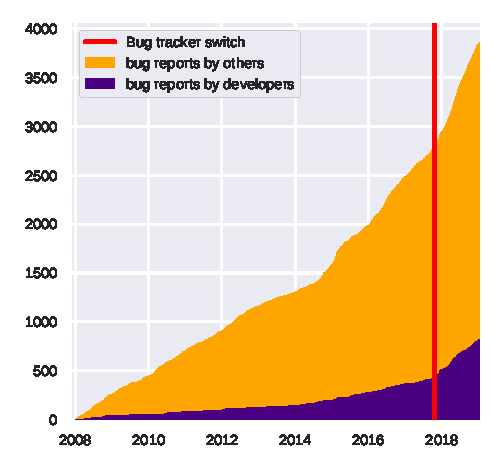
\includegraphics{cumulative_bugs.eps}
%\caption{Cumulative number of bug reports (since 2008).} \label{cumulative_bugs}
%\end{figure}

%\begin{figure}
%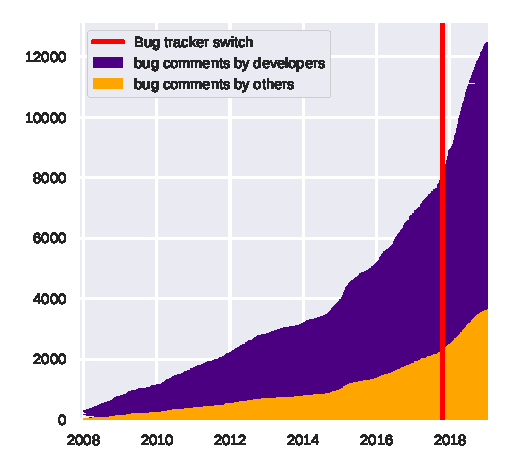
\includegraphics{cumulative_comments.eps}
%\caption{Cumulative number of comments (since 2008).} \label{cumulative_comments}
%\end{figure}

%\subsection{Influence of new releases}
%\label{influence_release}

%\paragraph{Influence on the number of bug reports}
%We expect release dates to be correlated to peaks of activity on the bug tracker, in particular peaks of new bug reports. Indeed, users will generally test new releases, for instance by trying to port preexisting projects to the new version, which might lead them to find new bugs (either regressions or bugs related to new features). In Fig.~\ref{bug_nb_with_releases}, we can see that while release dates are generally correlated to peaks of new bug reports by non-developers, this is not so much the case of reports by developers. We can also notice that beta releases are often correlated to higher peaks than final releases which is not surprising given that the users who test beta versions are more likely to be ready to report bugs, and beta versions are likely to be less polished.

%The highest peak is in 2015, after the first beta release of version 8.5. This was the first release in more than two years and it contained five big new features (``the result of five specific long-term projects''\footnote{Quote from:\\ \url{https://coq.inria.fr/distrib/V8.9.0/refman/credits.html\#credits-version-8-5}\\
%The next quotes are coming from the following sections of the same chapter of the Coq reference manual.}). Stabilizing these features and their (unplanned) interactions required more than a year of testing and three beta releases. The 8.5 release was both hard on developers, who found the release cycle too long, and on users, who were impacted by many compatibility issues. Consequently, a different approach was taken for the following releases: versions 8.6, 8.7 and 8.8 were ``developed on a time-based development cycle'' and contain ``the result of refinements, stabilization of features and cleanups of the internals of the system along with a few new features''. Attention was given to regression testing: changes were systematically tested by building a selection of the largest Coq projects. Therefore, it is not surprising that these frequent releases are correlated to smaller peaks of new bug reports.

%IMPORTANT: metre une phrase dans la partie description des variables qui indique qu'on fait 4 semaines pour celui la.
\begin{figure}
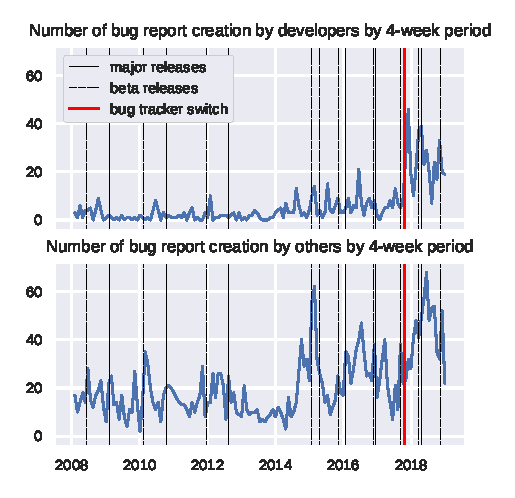
\includegraphics{bug_nb_with_releases.eps}
\caption{Number of issues per day (averaged by 4-week periods) with release dates (since 2016).} \label{bug_nb_with_releases}
\end{figure}

%\paragraph{Influence on the number of comments}
%In Fig.~\ref{comments_with_releases}, we can see that release dates are correlated to peaks of comments by developers (and not so much by other people). This is explained by the fact that bug reports are generally answered by developers, thus any peak in bug reporting is bound to induce a peak in bug commenting by developers.

\begin{figure}
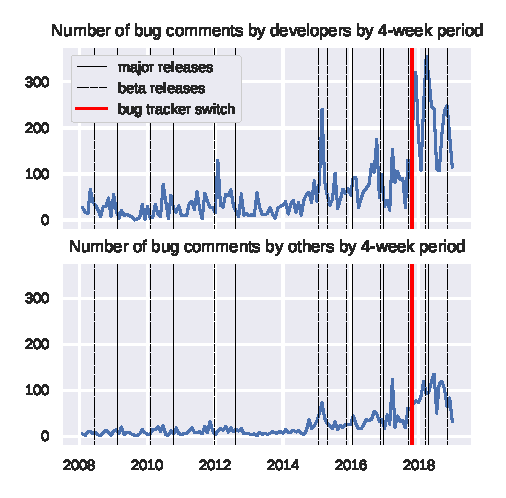
\includegraphics{comments_with_releases.eps}
\caption{Number of comments per day (averaged by 4-week periods) with release dates (since 2016).} \label{comments_with_releases}
\end{figure}

\begin{figure}
\includegraphics{reporters_with_releases.eps}
\caption{Number of weekly distinct reporters (averaged by 4-week periods) with release dates (since 2016).} \label{reporters_with_releases}
\end{figure}

\begin{figure}
\includegraphics{commentators_with_releases.eps}
\caption{Number of weekly distinct commentators (averaged by 4-week periods) with release dates (since 2016).} \label{commentators_with_releases}
\end{figure}

\section{Methodology}
\label{methodology}

\subsection{Quantitative}
We exploit the fact that the switch from Bugzilla to GitHub can be seen as a clear cutoff in time to use a temporal sharp Regression in Discontinuity design (RDD) to estimate the effects of the switch on our outcome variables; to determine if these estimated effects are statistically significant; and to interpret these effects in a causal way. 
The idea behind RDD is that factors that influence bug reporting activity are fairly similar just before and just after the cut-off point, which makes the changes observed between just after and just before the cut-off a consequence of the change that occurred at the cut-off (i.e., the switch of bug reporting platform).

The assumption behind this analysis is that bug reporters did not choose the exact moment in which the switch would take place. In the absence of any other discontinuity, the changes in the behavior of bug reporters just before and just after the migration is likely to depend mainly on the switch: the other factors influencing bug reports evolve slowly, and should be pretty similar just before and just after the switch. It is important to note that estimated effects using this method will inform of the effect near the threshold (i.e., it will only give the Local Average Treatment Effect --LATE-- of the switch). Indeed, in the same way that behavior just before and just after the threshold is not likely to be different in the absence of the switch, the behavior several periods before and several periods after is likely to be different even in the absence of the switch. See~\cite{angrist2014mastering} and~\cite{angrist2008mostly} for an accessible and intuitive introduction to Regression on Discontinuity analysis; and~\cite{lee2010regression} and~\cite{jacob2012practical} for further details and a practitioner's guide to its empirical application.

We model the evolution of the bug reporting behaviour around the switch by two different functions, one before and one after the switch, fitted using ordinary least squares. Their purpose is to accurately estimate the value at the switch in the absence and presence of treatment. Since only their value around the cutoff point is relevant, we can choose to estimate them on a restricted bandwidth (number of periods) around the cutoff, or on a larger dataset. We also have the choice of different functional forms for these models.

In the context of a Regression in Discontinuity analysis, the choice of the bandwidth of the analysis and the functional form of the regression is always difficult. On the one hand, including data points that are far from the cut-off (in our case the switch) will increase precision as it will reduce standard errors (because we will have more data points). On the other hand, however, including those points can bias estimation near the cut-off if the functional form of the evolution in the absence of switch is not accurately specified. Our main specification takes a conservative approach with a relatively small bandwidth of 180 days before and after the switch to minimize possible bias, and a comparatively simpler linear model. However, as a robustness check, we also estimate a quadratic model on a larger time frame (455 days on each side). This conservative approach reduces the statistical power of our analysis, increasing the probability of observing false negatives (being unable to detect an effect where such an effect exists).

We use time as rating variable\footnote{The rating variable is also sometimes called the running variable or the forcing variable in the literature.} (with the cutoff centered at zero) and we estimate the following regression:  
\begin{equation*}
\arraycolsep=0pt
\begin{array}{l}
\mbox{\emph{Number of bug reports}}_t = \\
\quad\quad \gamma_0 +\gamma_1 \times \mbox{\emph{Relative date}}_t
+ \gamma_2 \times \mbox{\emph{After switch}}_t \\
\quad\quad +~\gamma_3 \times \mbox{\emph{Relative date}}_t \times \mbox{\emph{After switch}}_t
+ \epsilon_t
\end{array}
\end{equation*}
\noindent where $\mbox{\emph{Number of bug reports}}_t⁡$ is the total number of bugs reported during the day $t$; $\mbox{\emph{Relative date}}_t$ is the number of days from the date of the switch (zero is the first period after the switch); $\mbox{\emph{After switch}}_t$ is a binary variable equal to one if $t$ is a period after the switch and zero otherwise; $\mbox{\emph{Relative date}}_t \times \mbox{\emph{After switch}}_t$ is called the interaction term and $\epsilon_t$ is the residual error. This is equivalent to estimating the following two regressions, respectively before and after the switch:
\begin{equation*}
\begin{array}{l}
\mbox{\emph{Number of bug reports}}_{t < 0} ⁡=\\
\quad\quad \gamma_0 + \gamma_1 \times \mbox{\emph{Relative date}}_t + \epsilon_p \medskip\\
\mbox{\emph{Number of bug reports}}_{t \geq 0} = \\
\quad\quad (\gamma_0 + \gamma_2) + (\gamma_1 + \gamma_3) \times \mbox{\emph{Relative date}}_t + \epsilon_t
\end{array}
\end{equation*}
We estimate this regression by Ordinary Least Squares~\cite{wooldridge2015introductory} and compute heteroscedasticity robust standard errors.\footnote{The errors $\epsilon_t$ are said to be heteroscedastic if their variances differ. The standard calculations for estimation errors assume equal variances~\cite{wooldridge2015introductory}.
} Coefficient $\gamma_0$ is the estimated value just before the cutoff and $\gamma_1$ the slope before the cutoff. Coefficients $\gamma_2$ and $\gamma_3$ are the estimates of interest and will tell us the jump of the number of bugs reports just after the switch and the change in slopes due to the switch respectively. 

We estimate this regression for two different sub-samples: the developers and the non-developers. We replicate this analysis for all our outcome variables by changing the variable on the left hand side of the equation. 

\subsection{Qualitative}

In order to obtain qualitative insights into the effects of the switch that will help us put in context and interpret the quantitative results, we conducted semi-structured interviews of all developers of Coq that were active at the time of the switch (with the exception of the developer that conducted the migration). A total of 9 interviews were conducted between 19th March and 4th April 2019. Some were done face to face and the others by video-conference with an average length of 33.5 minutes per interview. Both authors were present during the interviews and all the interviews were recorded. Some basic questions were asked to all of the interviewees and according to the answers some additional questions were also asked. The answers were coded by both authors in an attempt to minimize errors. Code and questions can be found in the supplementary material. 

\section{Results}
\label{results}
\subsection{Impact on the number of bug reports}

\begin{table}
\centering
\caption{Estimated impact of the switch on the number of issues. Coefficients are highlighted if they are statistically significant with $p<0.1$ ($\dagger$), $p<0.05$ (*), $p<0.01$ (**) or $p<0.001$ (***). Standard error is in parentheses.}
\label{tab:bug_nb}
\begin{tabular}{|r|c|c|c|}
\hline
&  Total & Developers & Non-developers \\
\hline
$\mbox{\emph{After switch}}_p$ & 0.629 & \textbf{0.73**} & -0.101 \\
 & (0.354) & (0.239) & (0.244) \\
\hline
$\mbox{\emph{Relative date}}_p$ & 0.00114 & -0.000383 & 0.00152 \\
$\times \mbox{\emph{After switch}}_p$ & (0.00341) & (0.00227) & (0.00245) \\
\hline
$\mbox{\emph{Relative date}}_p$ & 0.00305 & -0.00013 & \textbf{0.00318*} \\
 & (0.00182) & (0.000816) & (0.00157) \\
\hline
Constant & \textbf{1.23***} & \textbf{0.269***} & \textbf{0.96***} \\
 & (0.21) & (0.0809) & (0.181) \\
\hline
Observation number & 350 & 350 & 350 \\
\hline
\end{tabular}
\end{table}

\begin{figure}
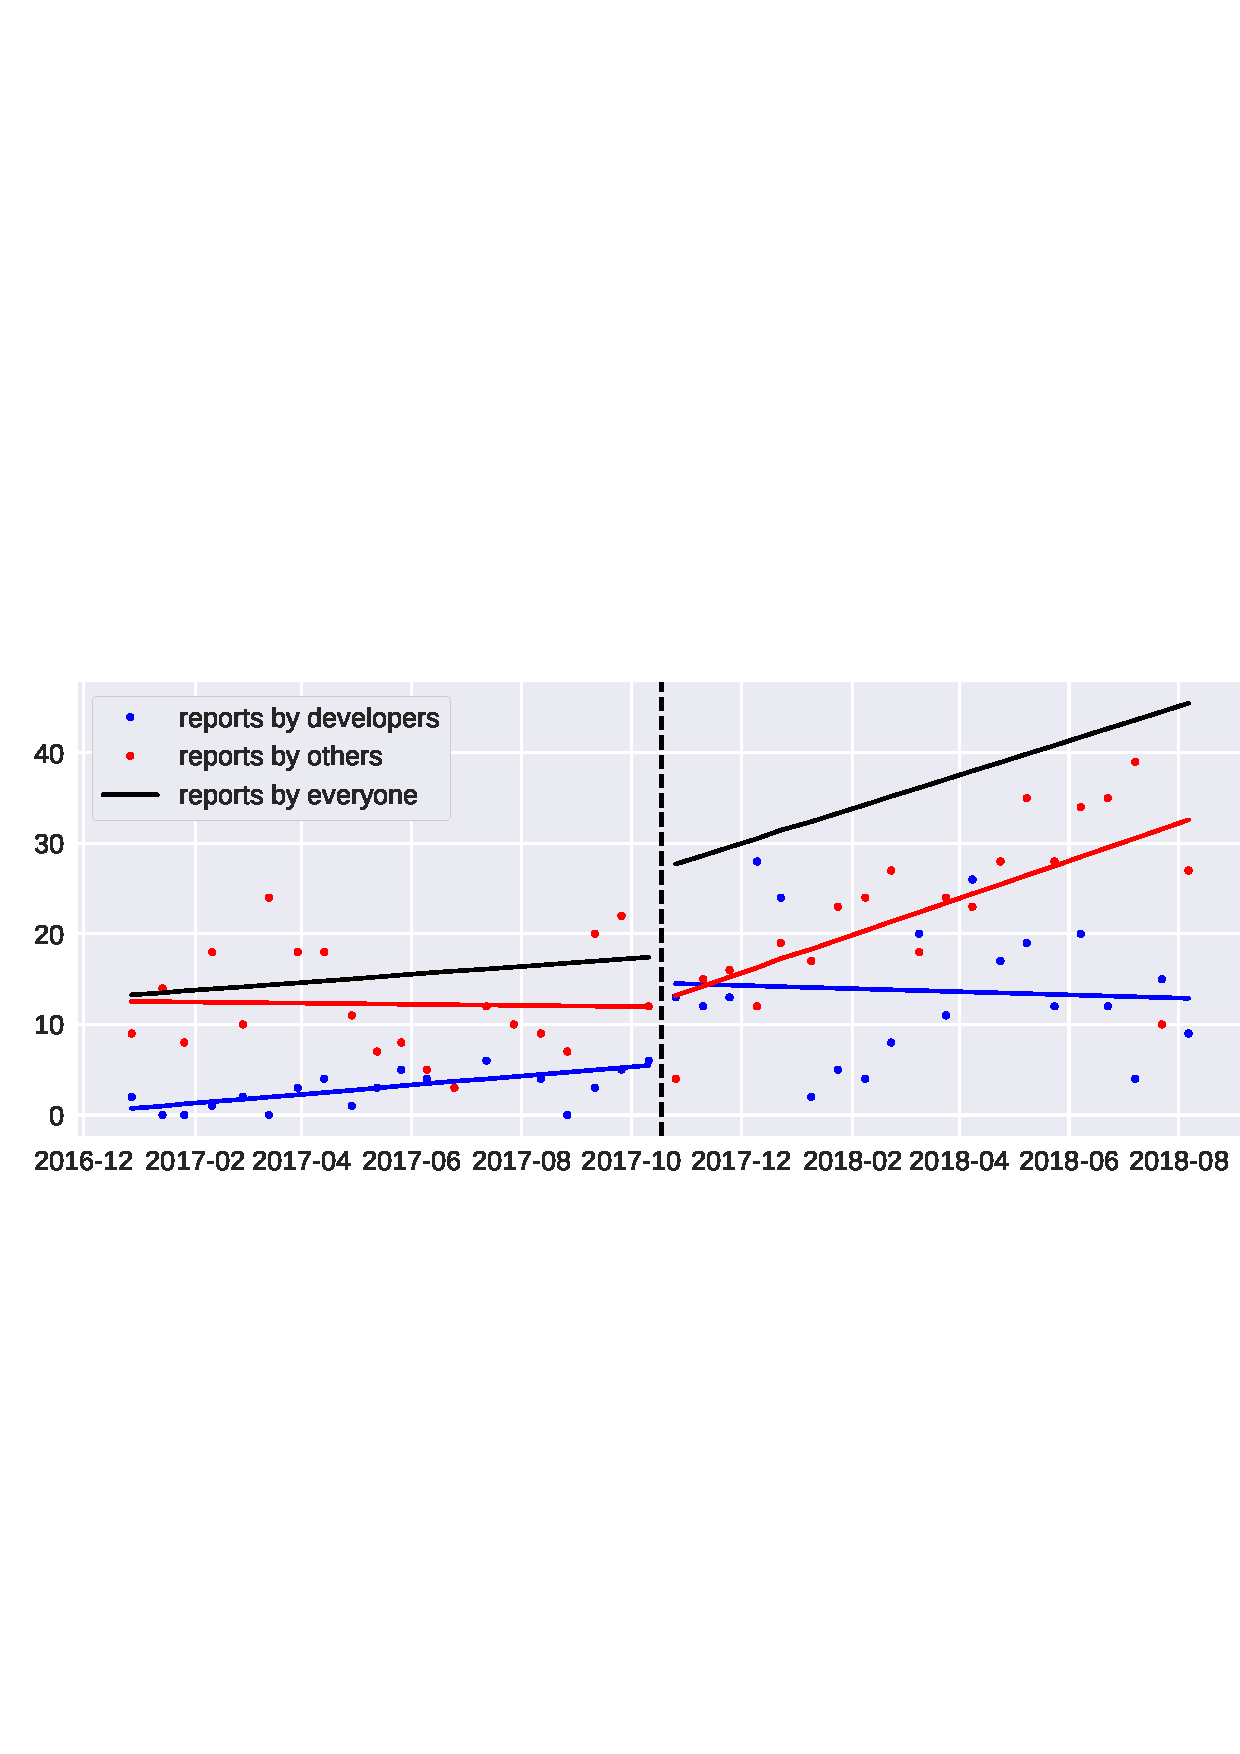
\includegraphics{bug_nb_rd.png}
\caption{Number of issues per day before and after the migration (with fitting lines and confidence intervals from the regression results, and points corresponding to average values over two-week periods).} \label{bug_nb_rd}
\end{figure}

Table~\ref{tab:bug_nb} presents the estimated impact of the switch on the number of reported bugs. Each column shows the estimates for a different sub-sample (i.e., all bug reporters, developers and non-developers). Asterisks represent different classical levels of statistic significance. We interpret results as significant if the p-value is below 0.1. Estimates that are not statistically significant cannot be interpreted as an absence of effect but indicate that if such effect occurred, we are unable to discern it with our conservative approach. Fig.~\ref{bug_nb_rd}  shows the number of reported bugs before and after the switch and the fitting lines and confidence intervals corresponding to the regression results. 

For developers, we see a statistically significant positive jump in bug reports just after the switch. In particular changing the bug reporting platform is estimated to have increased the daily number of reported bugs by 0.7 (representing an increase of around 250\%). That is, on average, we observe around one bug reported by developers every day after the switch, %(but close to the switch)
while before the switch developers reported a bug every three days. There is no statistically significant effect on the number of bug reports by other contributors: we cannot reject that such a variation occurred, but we are unable to discern it with our conservative approach.

\subsection{Impact on the number of distinct bug reporters}

Table~\ref{tab:reporters} and Fig.~\ref{reporter_nb_rd} show the estimated impact of the switch on the number of distinct bug reporters each week. These results demonstrate that the switch to GitHub positively affected not just the number of bug reports but also the number of distinct developer bug reporters in a given week. The number of distinct developers that reported bugs in a given week increased by around 130\% (from a 1.5 reporting developers each week before the switch to 3.42 after)

\begin{table}
\centering
\caption{Estimated impact of the switch on the number of distinct reporters each week. Coefficients are highlighted if they are statistically significant with $p<0.1$ ($\dagger$), $p<0.05$ (*), $p<0.01$ (**) or $p<0.001$ (***). Standard error is in parentheses.}
\label{tab:reporters}
\begin{tabular}{|r|c|c|c|}
\hline
&  Total & Developers & Non-developers \\
\hline
$\mbox{\emph{After switch}}_p$ & 2.17 & \textbf{1.92*} & 0.245 \\
 & (1.68) & (0.977) & (1.27) \\
\hline
$\mbox{\emph{Relative date}}_p$ & 0.146 & 0.0162 & 0.13 \\
$\times \mbox{\emph{After switch}}_p$ & (0.108) & (0.0648) & (0.0862) \\
\hline
$\mbox{\emph{Relative date}}_p$ & 0.0608 & -0.00462 & 0.0654 \\
 & (0.0903) & (0.0378) & (0.0675) \\
\hline
Constant & \textbf{6.03***} & \textbf{1.5**} & \textbf{4.53***} \\
 & (1.47) & (0.579) & (1.11) \\
\hline
Observation number & 50 & 50 & 50 \\
\hline
\end{tabular}
\end{table}

\begin{figure}
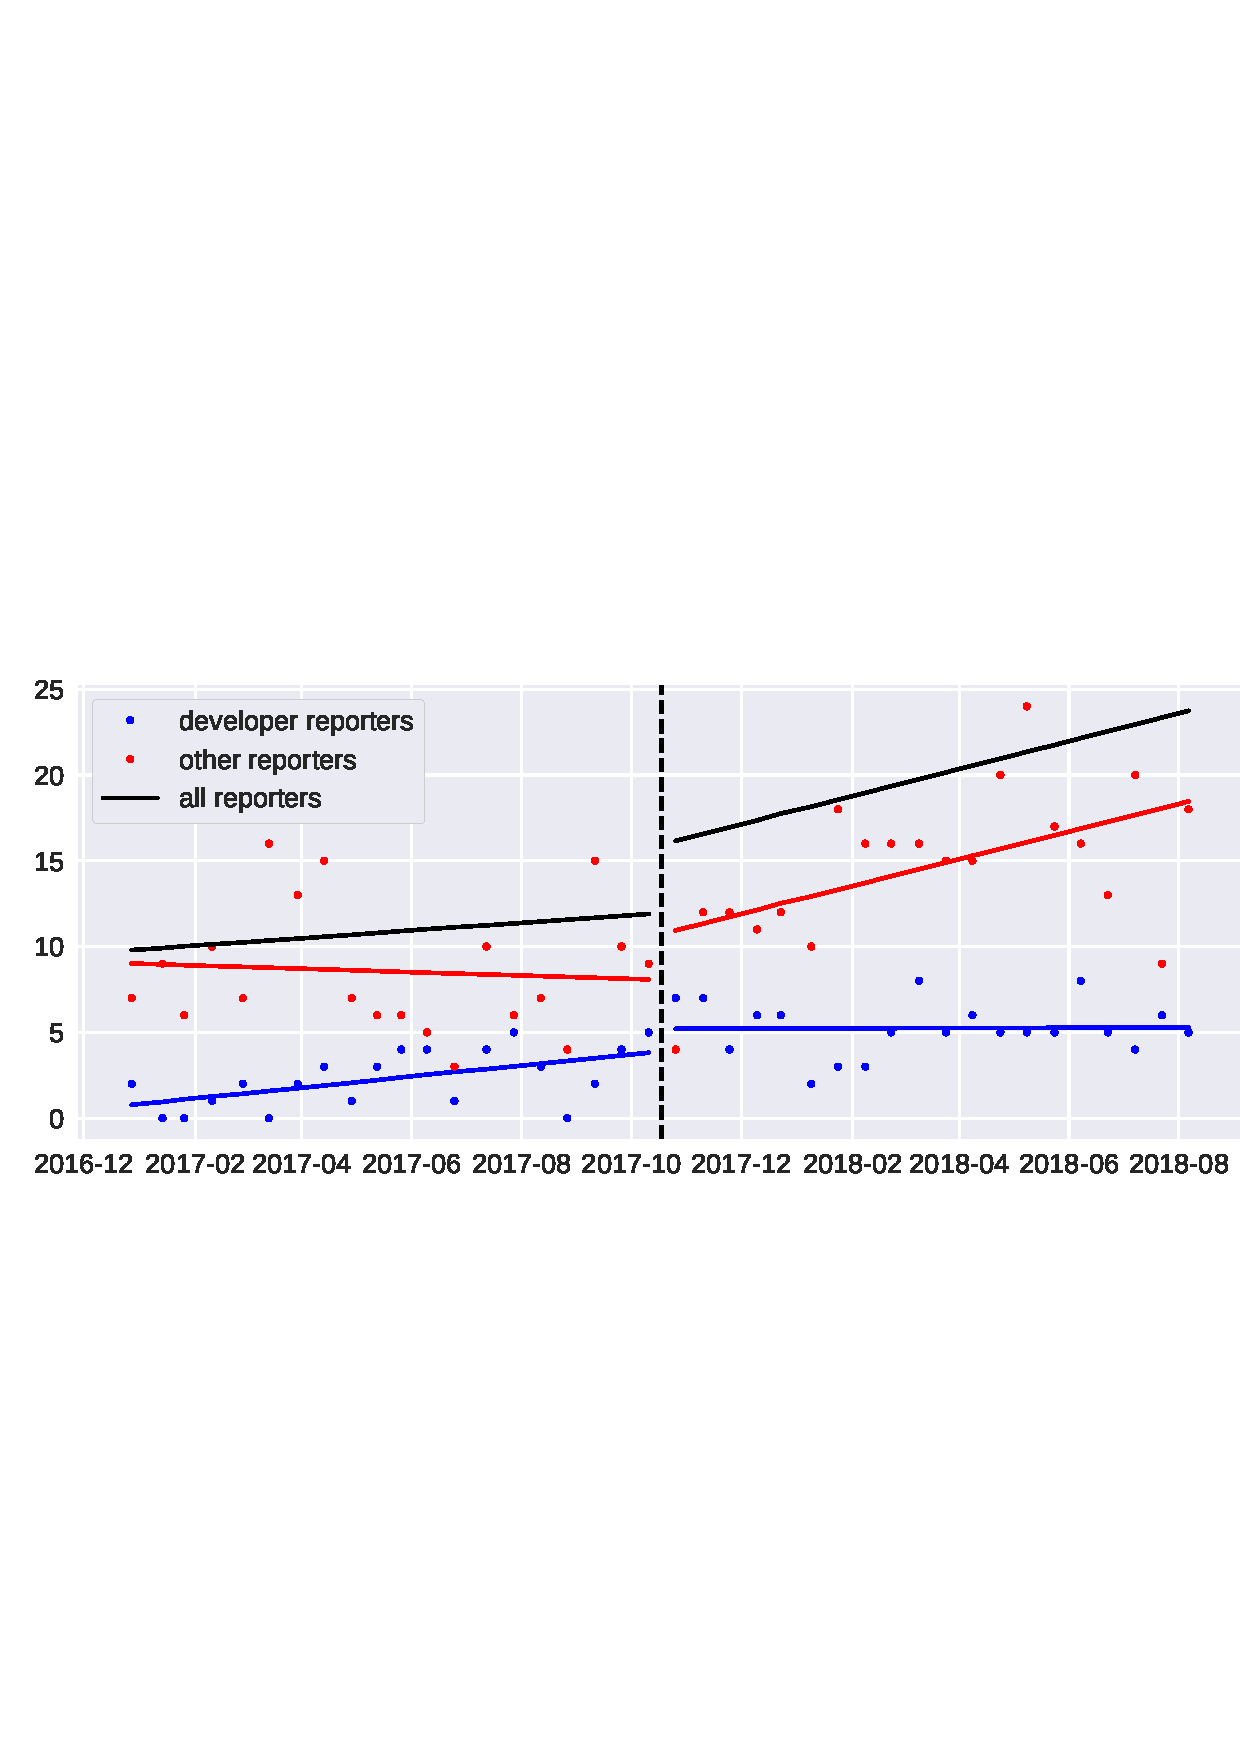
\includegraphics{reporter_nb_rd.png}
\caption{Number of weekly distinct reporters before and after the migration (with fitting lines and confidence intervals from the regression results, and points corresponding to average values over two-week periods).} \label{reporter_nb_rd}
\end{figure}

\subsection{Impact on the number of comments}

Table~\ref{tab:comment_nb} and Fig.~\ref{comment_nb_rd} show the estimated impact of the bug tracker switch on the number of comments. We see a statistically significant jump in the number of comments, which more than doubles (from 4.8 comments per day before the switch to 10.3 after the switch). This appears to be, for the most part, due to comments by developers who increased their average number of comments per day from around 3 before the switch to around 8 after.

\begin{table}
\centering
\caption{Estimated impact of the switch on the number of comments. Coefficients are highlighted if they are statistically significant with $p<0.1$ ($\dagger$), $p<0.05$ (*), $p<0.01$ (**) or $p<0.001$ (***). Standard error is in parentheses.}
\label{tab:comment_nb}
\begin{tabular}{|r|c|c|c|}
\hline
&  Total & Developers & Others \\
\hline
$\mbox{\emph{After switch}}_p$ & 5.5* & 4.76** & 0.739 \\
 & (2.24) & (1.79) & (0.717) \\
\hline
$\mbox{\emph{Relative date}}_p$ & 0.0155 & 0.0144 & 0.00112 \\
$\times \mbox{\emph{After switch}}_p$ & (0.0205) & (0.017) & (0.0063) \\
\hline
$\mbox{\emph{Relative date}}_p$ & 0.00147 & -0.00288 & 0.00435 \\
 & (0.00882) & (0.00673) & (0.00383) \\
\hline
Constant & 4.77*** & 2.95*** & 1.82*** \\
 & (1.03) & (0.704) & (0.463) \\
\hline
Observation number & 360 & 360 & 360 \\
\hline
\end{tabular}
\end{table}

\begin{figure}
\includegraphics{comment_nb_rd.png}
\caption{Number of comments per day before and after the migration (with fitting lines and confidence intervals from the regression results, and points corresponding to average values over two-week periods).} \label{comment_nb_rd}
\end{figure}

\subsection{Impact on the number of distinct commentators}

Table~\ref{tab:commentators} and Fig.~\ref{commentator_nb_rd} show the estimated impact of the bug tracker switch on the number of distinct commentators each week. We can see a statistically significant jump in the total number of commentators, in the number of developer commentators, and in the number of non-developer commentators.

In general terms, the number of distinct commentators in a given week changed from an average of 7 to an average of 13 (almost doubling the commentators). Analyzing the developers and the non-developers, we can see that this increase is due in larger part to non-developers (whose number of commentators more than doubles) while, among developers, this number increases by 66\%.

\begin{table}
\centering
\caption{Estimated impact of the switch on the number of distinct commentators each week. Coefficients are highlighted if they are statistically significant with $p<0.1$ ($\dagger$), $p<0.05$ (*), $p<0.01$ (**) or $p<0.001$ (***). Standard error is in parentheses.}
\label{tab:commentators}
\begin{tabular}{|r|c|c|c|}
\hline
&  Total & Developers & Non-developers \\
\hline
$\mbox{\emph{After switch}}_p$ & 6.19*** & 2.53* & 3.66** \\
 & (1.81) & (1.05) & (1.17) \\
\hline
$\mbox{\emph{Relative date}}_p$ & 0.205$\dagger$ & 0.0769 & 0.128 \\
$\times \mbox{\emph{After switch}}_p$ & (0.118) & (0.0641) & (0.0924) \\
\hline
$\mbox{\emph{Relative date}}_p$ & -0.0692 & -0.0469 & -0.0223 \\
 & (0.0833) & (0.0589) & (0.0463) \\
\hline
Constant & 7.06*** & 3.83*** & 3.23*** \\
 & (1.54) & (0.984) & (0.861) \\
\hline
Observation number & 50 & 50 & 50 \\
\hline
\end{tabular}
\end{table}


\begin{figure}
\includegraphics{commentator_nb_rd.png}
\caption{Number of weekly distinct commentators before and after the switch (with fitting lines and confidence intervals from the regression results, and points corresponding to average values over two-week periods).} \label{commentator_nb_rd}
\end{figure}

\section{Discussion}
\label{discussion}

\subsection{H1: impact on the number of reported bugs}

We hypothesized that the switch to a platform that is perceived as more modern and easier to use would increase the number of reported bugs. Our data analysis only shows such an effect on the number of bug reported by developers, and not on the bugs reported by non-developers, which only partially validates our first hypothesis.

The developers were using the bug tracker very little before the switch. This means that when they found bugs in the course of the development, they stored them in personal task lists, fixed them immediately, or tried to remember them in their heads until they could fix them (likely with some bugs being forgotten in the process). Meanwhile, they were discussing a lot through the pull request system on GitHub. The move of the bug tracker to GitHub made it closer to the main development platform (the repository where pull requests are submitted and reviewed), both in terms of location and in terms of user interface. These reasons are probably what pushed developers to use it more.

The increased use of the bug tracker in place of personal task lists makes the whole development process more transparent and is likely to be beneficial to new contributors.

If it is the case that the switch had no effect on the number of bugs reported by non-developers, this could mean that when people decide to report bugs, they do so before accessing the bug tracker, and nor the requirement of creating an account, nor the heavier and less modern interface, are sufficient to discourage them.

%The second one is that more people intended to report bugs but this increase was blurred out by a simultaneous decrease in the number of duplicate bug reports, thanks to the better search provided by GitHub. People intending to report a bug and finding out that it was already reported would post a comment (although if this was frequently the case, there should be an increase in the number of comments by non-developers, which hasn't been observed in a significant way neither) or add a reaction (GitHub feature allowing to up-vote a comment) or leave without taking any action instead. To confirm this second interpretation, we would need to analyze the impact of the switch on the number of bugs closed as duplicates.

\subsection{H2: impact on the pool of reporters and commentators}

% how many of the reporters of recent bugs had a GitHub account?

Having a common platform for the pull requests and the bug reports, and using a standard solution where a lot of users would already have an account, was hypothesized to have an impact on the pool of participants in the bug tracker. For non-developers, our data analysis only shows this effect in a statistically significant way on the number of commentators, which only partially validates our second hypothesis.

Analyzing deeper, we find that there exists not just a jump in the non-developer commentators in a given week but also a jump in the number of new non-developer commentators (i.e., people that had never before posted a comment). We show the results for the new commentators in the companion Jupyter notebook.

While we suggested that reporters would be motivated enough to not be affected by the bug tracking platform, this is less likely to be the case for people willing to comment. Furthermore, people who were already following the pull request activity were now subscribed to the bug tracking activity as well and this could have been enough to encourage them to post comments. The previous system made it harder and less flexible to subscribe to the bug tracker activity.

This analysis is consistent with previous findings: many people start by \emph{lurking} (i.e., mostly reading discussions) before starting to contribute to an open source project (for instance by participating to discussions)~\cite{von2003community}. In the context of GitHub, a significant portion of the new contributors start by \emph{watching} the repository (i.e., subscribing to its activity). These contributors contribute for longer periods and achieve a wider variety of contribution types, probably due to the knowledge and confidence they gained during the watching process~\cite{sheoran2014understanding}.

% Commenté pour faire plus court, et ça n'est pas suffisamment essentiel ici.
%These results are particularly interesting because they highlight an increase in the number of people involved in the development process in the large sense. They also show a remarkable change in the way non-developers engage in the software developing process following the switch.

The significant impact on distinct reporters and commentators among developers is more surprising but shows that some developers were disengaged from any kind of activity on the bug tracker before the switch. One developer explained this as a difficulty to keep track of activity on two platforms at once (GitHub for the pull requests and Bugzilla for the bug reports). Comparing data from pull request commentators and bug report commentators confirmed this: before the switch there were more developers commenting pull requests than bug reports in any given week, whereas after the switch this difference disappeared completely (graph available in the accompanying notebook).

%todo for future... are there more non-developers closer to become developers ?

\subsection{H3: impact on the interaction between users and developers}

The surge in the number of comments posted by developers shows that developers communicate more on the bug reports they receive, instead of just fixing and closing them. This result suggests once again that the switch was beneficial in terms of transparency of the development, an evolution that is likely to give greater satisfaction to the bug reporters and probably encourage engagement in the process of bug reporting and development more generally. Taken together with the increased number of non-developer commentators, this validates our third hypothesis.

% Commenté pour faire plus court, et ça n'est pas suffisamment essentiel ici.
Overall, these results suggest that the change of platform reinforced discussion among developers and among developers and non-developers, which may improve efficiency in the developing process, incentivize non-developers to have a more active role (maybe even assuming developing tasks) and in the long run increase the quality of the software (as bugs are probably better understood and fixed in better accordance to users' needs). 

\section{Threats to validity}
\label{threats}
\subsection{Internal validity and robustness checks}

The biggest concern that we have in our analysis is the fact that the date of the switch is close to the release date of a new version of Coq. The release of version 8.7.0 took place on October 17\textsuperscript{th}, and the migration on October 18\textsuperscript{th}. Then, the hypothesis that there is no other discontinuity around the threshold of interest does not completely hold in our case.
%First, we can argue that only our result on the number of comments by developers is threatened: the other statistically significant effects that we observed are not threatened because there is usually no peak in the corresponding variables after new releases.
%Second, we can also argue that there should have been a similar (or higher) peak in the month before the switch since the first beta of 8.7 had been released then (and beta releases generally result in higher peaks).
To confirm that it is not the migration that is driving our results, we do the exact same analysis that we do for the bug tracker switch, replacing the cutoff date by the date of all six major releases since 2009 (once we remove the latest release because we do not have yet enough data points after the release). We show that the only significant effect in the bug-tracker activity after a major release is the effect after the major release that match the switch. It is also, for the majority of the outcomes, by far the effect with the highest magnitude. 

%To provide some evidence that the date of the switch is not associated with an increase in the activity of open source software due to external factors (which will invalidate our results as explained before), we replicate our analysis for a comparable software: another French medium size open-source project: OCaml. We do not observe any increase in the bug-tracking activity for this project after the Coq bug-tracker switch date. If anything we see a decrease in activity so if there was an external factor that affected french open-source projects decreasing their activity. we will be underestimating the effect of the switch. 

%two robustness checks with our data. The first consists in removing the two weeks following the 8.7.0 release (and the switch) from our Regressions in Discontinuity. With these periods removed, the regressions still give very close results. The second consists in including a binary control variable that is equal to one if the period is in the two weeks after a release and zero otherwise. This control variable will capture the high peaks due to the release without the need of eliminating periods close to the switch. Again, our results remain very similar when we include this control variable. 

Our main specification for Regression on Discontinuity uses a small bandwidth and a linear model. In this section, we also present the results using all the available data (455 days on each side of the cutoff, corresponding to all the data that we collected after the switch and the same number of days before). To reduce the associated bias, we include a quadratic term to allow the regression to better fit the data and "adjust" to far away data points. Following Gelman et al. ~\cite{gelman2018high}, we include only a quadratic polynomial and not a polynomial of a higher order. Our results still hold with this specification. 

Temporal RDD have some notable differences with other types of RDD \cite{hausman2018regression}. One major difference is the capacity of anticipation and reaction to the treatment that affect directly the outcome. To overcome this potential problem, we redo our analysis with a donut RD (i.e. we exclude the data points just after and just before the migration, which are potentially problematic), following \cite{hausman2018regression}. Our results still hold with a slight decrease in the level of significativity but keeping the significativity at 10\%. 


%In order to corroborate that our results are not driven by activity occurring much after or much before the switching period (that is more likely to be affected by other factor beyond the switch), we check if our results are robust to the exclusion of the 1\%, 5\% and 10\% external values (i.e., values that are furthest from the switch) ~\cite{jacob2012practical}. 

%In the context of a Regression in Discontinuity analysis, the choice of the bandwidth (number of periods around the switch) of the analysis and the functional form of the regression is always difficult. By the one hand, including data points that are far from the cut-off (in our case the switch) will increase precision as it will reduce standard errors (because we will have more data points). By the other hand, however, including those points can bias estimation near the cut-off. In our preferred specification that we present in the results section, we take a conservative approach and take a relatively small bandwidth to minimize possible bias. In this section, we also present the results using all the disposable data. To reduce the associated bias, we include a quadratic term to allow the regression to better fit the data and "adjust" for far away data points. Following Gelman et al. (2018) ~\cite{gelman2018high}, we include only a quadratic polynomial and not a polynomial of a higher order.

%We also conduct one standard robustness check for Regression in Discontinuity analysis by changing the time window of the analysis to fifteen and to ten periods before and after the switch. Our main results are robust to these changes.
All results presented in this section can be found in the Jupyter notebook provided as a supplemental material. 
\subsection{External validity}

This is only a case study on a very specific project (by the target audience, the location and composition of its core team, etc.). We would really benefit from conducting similar analyses on other projects that went through a similar bug tracker switch.

We located another project that went through a similar switch from Bugzilla to GitHub and used the Bugzilla import tool with our modifications. It would have been a perfect case for replicating this analysis. A preliminary visualization of the data shows that, compared to the few years before the switch, there have been more bug reports and comments posted after the switch. Unfortunately, we learned that some data was lost during the crash of their previous bug tracker, which makes it really difficult to draw any reliable conclusion.
%after talking with the developer responsible for the migration, we learned that the switch was the consequence of a crash of the Bugzilla instance that could not be fixed, and that some data (bugs and comments) were lost in the crash. Some of it could be recovered and was manually added, which makes it inaccurately appear as activity after the switch.

We nonetheless believe that our conclusions can be generalized to some extent and encourage researchers to replicate this study, for instance using our migration tool and/or our analysis pipeline and methodology.

There is no reason to believe that these results would generalize to proprietary software projects. Some projects that are also less likely to benefit as much from a switch to GitHub are the larger projects (like Mozilla, Linux, Gnome, KDE, Apache) which have been using Bugzilla for a long time and have defined rigorous development processes, in particular regarding the use of the bug tracker. Coq is an example of a project that is developed in a very Bazaar-like fashion, with no clear rules on how to use the bug tracker, and this lack of rules was hindering the use of a complex bug tracker like Bugzilla. We believe that open source projects that share this lack of rules and this medium size are the more likely to benefit from a switch from Bugzilla (or similar bug trackers like Mantis), to GitHub (or the very similar GitLab platform), especially if they are already heavily using the latter for pull requests.

\section{Conclusion and perspectives}
\label{conclusion}
We have analyzed the impact of changing the bug reporting environment using a Regression in Discontinuity analysis with data from the switch of the Coq bug tracker from Bugzilla to GitHub.  We have shown that the switch incurred an increase in bug tracking activity in two ways. First, the developers are using the bug tracker more, to report their own bugs, and to discuss bug reports. Second, the non-developers are more numerous to take an active role by commenting bug reports as well. We find particularly interesting the change in the number of comments by developers and in the number of distinct non-developer commentators because it shows a shift in the dynamics of the bug reporting process that we believe can improve software development by engaging more people in the process, and by increasing openness and transparency.

Given the lack of literature on the effects of bug tracking environments, interested researchers could expand our analysis in many different ways. Analyzing other outcomes (such as pull requests or the rapidity of bug resolution) could give interesting additional insights and help create a more complete picture of the mechanisms at play.
% je pense qu'on peut se permettre d'enlever cette phrase maintenant
%It will be also interesting to analyze the effects on a longer period to see if the changes hold in the long run.
Replicating our analysis for different contexts and software would increase the external validity of the results.

Finally, we introduced and showed an example of the use of a Regression on Discontinuity design, that is novel in the context of empirical software engineering. We think that there are many cases where this methodology would be useful to help demonstrate causality from mined software repository data.

% Takeaways
% When to switch? It would be useful to come up with measures that indicate when a bug tracker is not adapted and a switch to another platform would be an improvement. (Or depending on specific objectives.)

\scriptsize
%\paragraph{}
\noindent \footnotesize{\textbf{Supporting data.}}
We provide our extraction and analysis code as a Jupyter notebook and the data we used as CSV files. We also provide the XML export of Bugzilla that was used for the migration and the migration script.
% XXXXX We also provide the interview questions and coding.
%Everything is available from \url{XXXXXXX}.
%\paragraph{}

%\noindent \footnotesize{\textbf{Authors' contributions.}}
%[masked for double-blind review]
%TZ found the research question, prepared and conducted the migration, designed and implemented the data extraction process, implemented the data analyses, and wrote part of the manuscript. AC designed the data processing and analyses, guided the implementation of the data analyses, presented the econometric method in use and wrote part of the manuscript.
%\paragraph{}

%\noindent\footnotesize{\textbf{Acknowledgements.}}
%We would like to thank Ambre Williams for valuable advice and help on the design and implementation of the data analyses and C\'ecile Rottner for general advice, support, and proof-reading.
%We would like to thank Andriy Berestovskyy for providing the Bugzilla import tool, and Martin Michlmayr for doing the first steps in porting our modifications upstream.

%
% ---- Bibliography ----
\bibliography{bib}
\bibliographystyle{IEEEtran}
%
\end{document}
